\documentclass[10pt,pdftex]{report}
\usepackage[T1]{fontenc}
\usepackage[utf8]{inputenc}
\usepackage[magyar]{babel}
\usepackage{graphicx}
\usepackage{amsmath}
\usepackage{amssymb}
\usepackage{multirow}
\usepackage{booktabs}
\usepackage{indentfirst}
\usepackage[a4paper]{geometry}
\usepackage{url}
\usepackage{titling}
\usepackage{float}
\usepackage{spverbatim}
\usepackage{xcolor}
\usepackage{hyperref}
\usepackage{adjustbox}
    \definecolor{titlebg}{RGB}{128,128,128}

\usepackage{lmodern}
\usepackage{etoolbox}
\patchcmd{\thebibliography}{\chapter*}{\section*}{}{}

\renewcommand{\thesection}{\arabic{section}}


\title{Hangsebesség mérése}

%% EZ ALÁBBI KÉT MEZŐT ÉRTELEMSZERŰEN KI KELL TÖLTENI
\author{Bíró Gergő Tamás}
\date{2025. március 4.}


%% FEJLÉC LEÍRÓ, NEM KELL MÓDOSÍTANI
\renewcommand*{\maketitle}{\noindent\colorbox{titlebg}{%
\parbox{\dimexpr\linewidth-2\fboxsep}{\color{white}%
\parbox{\linewidth}{\fontsize{18}{24}\selectfont\sffamily\bfseries\thetitle}%
}}\vskip 1em%
\begin{tabular}{l}%
Mérést végezte: \theauthor \\%
Neptunkód: R9SZLJ \\
Mérés dátuma: \thedate\\
Jegyzőkönyv végleges változata: \today %
\end{tabular}%
}
%%%%%%%%%%%%%%%%%%%%%

\begin{document}
\maketitle

%% ÉRDEMI MUNKA HELYE
\section*{A mérés célja}
A mérés elsődleges célja a hangsebesség kimérése, emellett még a mérés alatt célunk volt a Doppler-hatás kimutatása, valamint a hangsebesség hőmérséklettől vaó függésének a 
mérése, és ennek modellezése.
\section*{A mérési feladatok dokumentációja, az adatok kiértékelése és az eredmények értelmezése}
\subsection*{A mérés során használt eszközök}
\begin{itemize}
    \item{HC04 mérőmudul, 4 ehhez kötött hőmérő szenzor.}
    \item{Két ultrahangos kapszula.}
    \item{Rézcső, amiben a hang terjedését vizsgáljuk.}
    \item{Kád amely a rézcső egy szakaszát körbeveszi.}
    \item{Két vízforraló.}
    \item{Ventillátor.}
    \item{Oszciloszkóp.}
    \item{Mérőszalag.}
\end{itemize}
\subsection*{Mérés leírása}
Először az oszciloszkóp segítségével a mérőmodul által készített jelalakokat vizsgáljuk, ezután a csúsztatható ultrahangos kapszula minimális távolságra való beállítása mellet 
egy percig rögzítjük a mérőmodul által mért adatokat, ebből a hibás adatpontok kiszűréséhez létrehozunk egy szűrőrutint, amely a nagy mértékben kiugró adatokat eltávolítja az 
adatsorból. Ezután a hangsebesség meghatározásához 9 különböző távolságból, pozíciónként legalább 1-1 percig mérjük a terjedés idejét, a kapott adatokat megszűrjük, majd 
az egyes távolságokhoz tartozó adatokat átlagoljuk, a kapott átlagokra egyenest illesztünk, amelyből meghatározzuk a hangsebességet. Ezek után a ventillátor bekapcsoljuk 12V-os 
feszültség mellet, és nagyjából 20 percet várunk, amíg a csőben beáll a termikus egyensúly. MIután ez megtörtént a ventillátorba 3 különböző feszültséget táplálva mérjük a 
terjedési időket, amivel m,egpróbáljuk kimutatni a Doppler-hatást. Ezután kalibráljuk a hőmérőket, és feltöltjük a kádat vízzel. Miután a víz szintje túllépte a rézcsövet 
bekapcsoljuk a vízforralókat, és mérjük az adatokat, amíg a víz hőmérséklete nem éri el a 72$^{\circ} C$-t, ami után kihúzzuk a vízforralót, és miután elkezd csökkenni a víz 
hőmérséklete leállítjuk a mérést.
\subsection*{Mérési adatok kiértékelése}
\subsubsection*{Mérőmodul jelalakjainak vizsgálata}
Az alábbi adatok a csúsztatható kapszula minimális távolsága mellett lettek mérve.


A trigger jelének szélessége az oszciloszkóp kurzorával leolvasva $10.30\mu s\pm0.10\mu s$-nek adódott, amely jelentős mértékben eltér az elméleti $15\mu s$ értéktől.
A trigger jelét ábrázolva megfigyelhetjük, hogy a jel valóban négysög alakú, maximális nagysága nagyjából $0.35V$.
\begin{figure}[H]
    \centering
    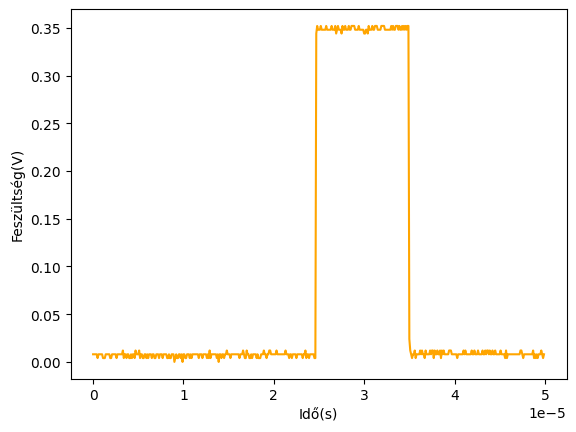
\includegraphics[scale=0.5]{./Trigger.png}
    \caption{Trigger jele.}
\end{figure}
Az dó jele 8 darab az oszciloszkóp kurzorával mérve $12.00\mu s\pm 0.40\mu s$ széleségű négyszögjelből áll.
\begin{figure}[H]
    \centering
    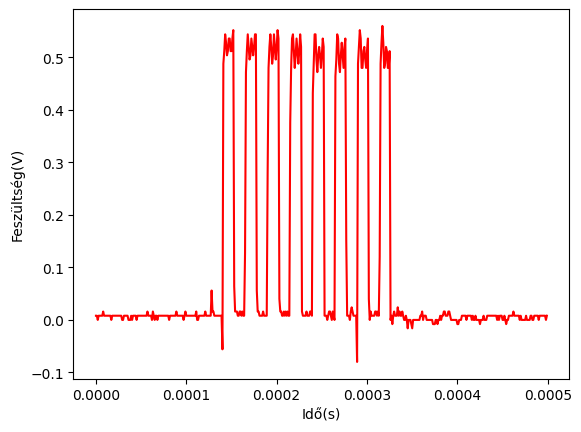
\includegraphics[scale=0.5]{./Ado.png}
    \caption{Adó jele.}
\end{figure}
Az adó jelében megfigyelhető impulzusok között van egy-egy nagyjából szintén $12\mu s$-os időszak, amikor a kimenő jel feszültsége közel elhanyagolható. 
Amennyiben ez a mintázat időben folyamatosan ismétlődne, és nem csak mérési ciklusonként 8-szor akor ennek a jelnek a frekvenciája $41667Hz$ lenne, amely közel van a 
kapszula ideális átviteli frekvenciájához, amely $40hHz$. 
\newline
\newline


A vevő jelét megfigyelve egy amplitúdómodulált jelet láthatunk, amelynek fél periódusának szélessége, $12\mu s \pm 1\mu s$ amely megegyezik az adó által kibocsájtott 
impulzusok szélességével.
\begin{figure}[H]
    \centering
    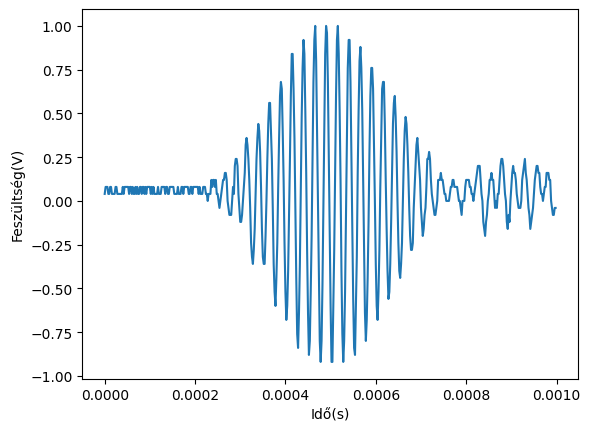
\includegraphics[scale=0.5]{./Vevo.png}
    \caption{Vevő jele.}
\end{figure}
Azonban láthatjuk, hogy a vevő teljes jele szélesebb, mint az adóé, amely feltehetőleg amiatt van, hogy a kibocsájtott ultrahang nem csak a levegőben, hanem a cső anyagában 
is terjed, a csőben lévő rezgések máskor érik el a vevő kapszulát, mint a levegőben terjedő hullám, így összességében a vevő jele szélesebb lesz, mint az adóé.
\begin{figure}[H]
    \centering
    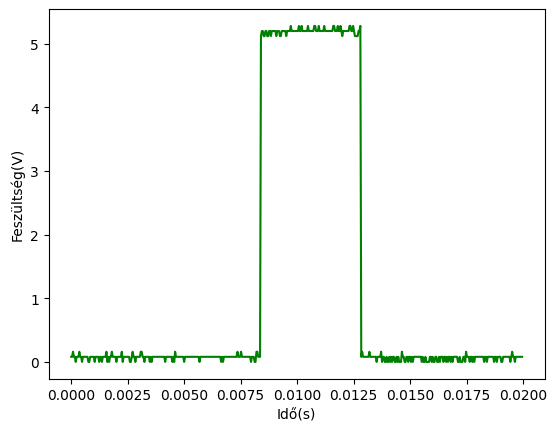
\includegraphics[scale=0.5]{./Echo.png}
    \caption{Echo jele.}
\end{figure}
Az echo jel szélessége az oszciloszkópon mérve a jelenlegi elzendezésben $4.44ms\pm0.04ms$, amennyiben az echo jelét az adó és a vevő jelével egyszerre ábrázoljuk azt figyelhetjük meg, 
hogy az echo jele az adó jelénekvégével kezdődik, és az adó jelének kezdetével végződik.
\begin{figure}[H]
    \centering
    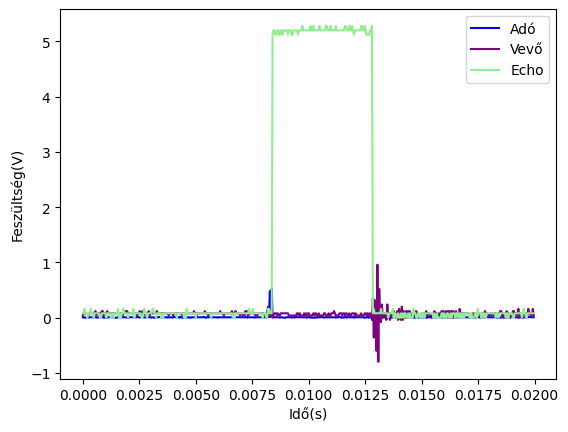
\includegraphics[scale=0.5]{./AVE.png}
    \caption{Echo, adó és vevő jeleinek helyzete az időben egymáshoz képest.}
\end{figure}
Egy a mérőpanelen elíndított rövid nagyjából 30 másodperces mérésből származó mérésből kapott idők átlaga $4.445ms$-nek adódik, amely szinte teljesen megegyezik az echo jel 
szélességével, amit az oszciloszkópon mértünk, így feltételezhetjük, hogy a berendezés aterjedési időket az echo jel szélességéből méri, amely valóban a heng indítása, és 
érkezése között eltelt idővel egyenlő.
\newline

Az alábbiakban a fentiek jobb szemléltetéséhez még további ábrák lesznek láthatóak, azonban amennyiben azokon ábrázolva van a trigger feszöltsége a mérést indító négyszögjel nem 
lesz rajta látható, mivel jel rögzítése rossz pillanatben lett indítva, aminek hatására az impulzus már nem látható benne.
\begin{figure}[H]
    \centering
    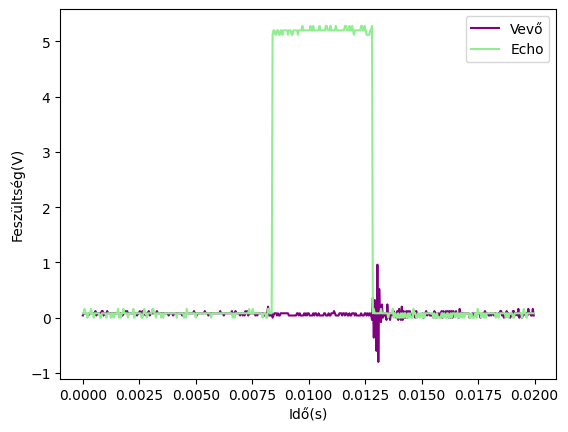
\includegraphics[scale=0.5]{./VE.png}
    \caption{Vevő, és adó jelei.}
\end{figure}
\begin{figure}[H]
    \centering
    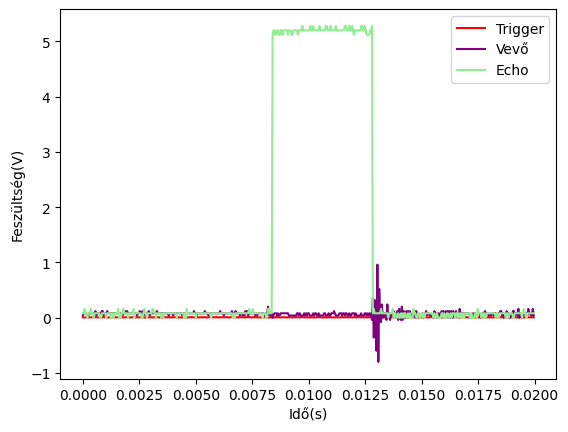
\includegraphics[scale=0.5]{./TAE.png}
    \caption{Trigger adó, és echo jelei.}
\end{figure}
\begin{figure}[H]
    \centering
    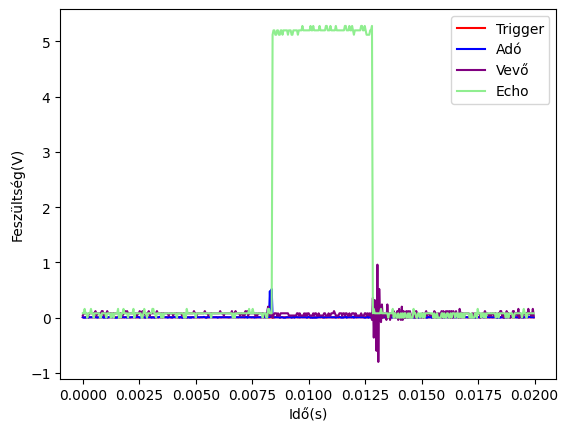
\includegraphics[scale=0.5]{./TAVE.png}
    \caption{Echo, adó, trigger és vevő jelei.}
\end{figure}
\subsubsection*{Alapvonalon történő mérés}
A csúsztatható kapszulát a minimális távolságon tartva 1 percnél kicsivel hosszabb mérést indítunk. A mérés során kapott időadatokat ábrázolva láthatjuk, hogy a jelek negyja 
egy sávba esik, vagy attól csak viszonylag kis mértékben tér el, azonban megfigyelhető még egy rithább sáv, amely az előző sávtól negyjából 12$\mu s$-re tér el, hasonló adatot 
kapunk az idő adatok szórásának kiszámításából is, amely $12.14\mu s$-os szórásértéket ad. Ez az időkülönbség megegyezik az adó jelének egy impulzusának szélességével, valamint 
a vevő jelének fél periódusával, így ebből arra lehet következtetni, hogy a sávosságot az idézi elő, hogy a mérőpanel  a vevő jelét egy periódussal később detektálja a kelleténél 
így az echo jel hossza megnő nagyjából 12$\mu s$-al, így a mmért didőben is megjelenik egy ekkora eltérés.
\begin{figure}[H]
    \centering
    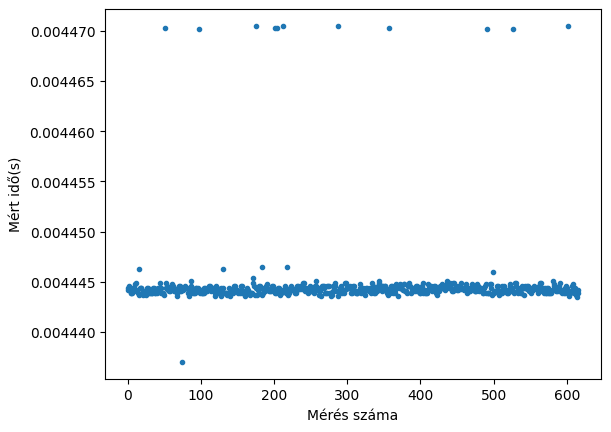
\includegraphics[scale=0.5]{./Alapvonal_szuretlen.png}
    \caption{Alapvonalon mért iddők a mérés számának függvényében.}
\end{figure}
\subsubsection*{Szűrőrutin}
A fent tapasztalt egy periódussal való elcsúszás kiküszöbölésére jó megoldás lehet, ha a mért adatokat megszűrjük úgy, hogy a valós értéktől jelentősen eltérő adatsorokat 
eltávolítjuk a mért adatok közül. Az ehhez használt algoritmus jelenleg a következőket fogja csinálni:
\begin{enumerate}
    \item{A bemeneti érték egy numpy array, amelynekegy elemében egy méréshez tartozó mért adatok vannak}
    \item{Az összes mért adatot a mért idő szerint növekvő sorba rendezzük.}
    \item{Leolvassuk a rendezett adatok harmadánál elhelyezkedő adatponthoz tartozó időt, ezt fogjuk a valós időnek tekinteni a szűrés során.}
    \item{Visszatérési értéknek veszünk egy listát, ami nem tartalmazza azokat az adatpontokat, amelyeknek a mért ideje 5$\mu s$-nél nagyobb mértékben tér el a valósnak 
    tekintett időtől.}
\end{enumerate}
Az algoritmushoz tartozó python kód a következő lesz:
\begin{spverbatim}
    def szuro(x):
    rendezett = x[x[:,0].argsort()]
    minta_ertek = rendezett[:,0][int(len(x)/3)]
    eredmeny = [i for i in rendezett if (i[0] <= minta_ertek + 5 and i[0] >= minta_ertek - 5)]
    return eredmeny
\end{spverbatim}
Az alapvonalon mért adatokon a szűrőrutint futtatva megfigyelhetjük, hogy valóban sikerült megszűntetni az adatpontok sávosságát.
\begin{figure}[H]
    \centering
    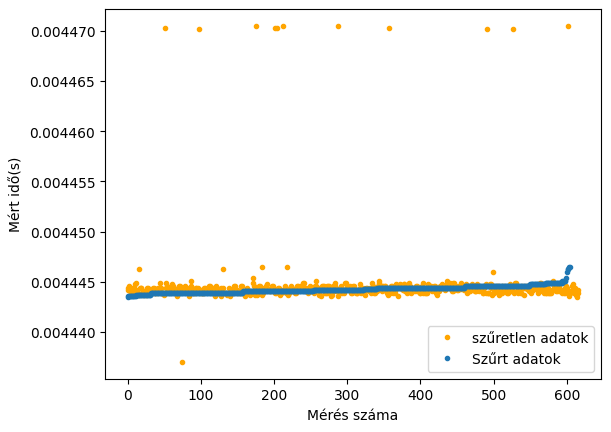
\includegraphics[scale=0.5]{./Alapvonal_szurt.png}
    \caption{Alapvonalon mért iddők a szűrés előtt, és után.}
\end{figure}
A szűrés után az adatokat hisztogrammon ábrázolva a követketkező eloszlást láthatjuk:
\begin{figure}[H]
    \centering
    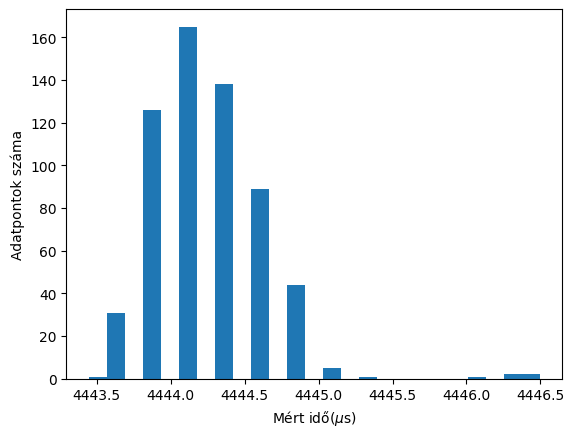
\includegraphics[scale=0.5]{./Alapvonal_hisztogramm.png}
    \caption{Alapvonalon mért iddők eloszlása a szűrés után.}
\end{figure}
A fent látható eloszlás egy normál eloszlásnak, a szórását kiszámolva pedig arra jutunk, hogy az a szűrés előtti $12.140\mu s$-ról $0.139\mu s$-ra csökkent.
\subsubsection*{Hangsebesség meghatározása}
A alábbiakban a méréseket több különböző távolságban végeztük az alapvonaltól, mindegyik mérési sorozat legalább 1 percig tartott, a kapott adatokat a fent leírt 
szűrőrutin segítségével megszűrtük, majd a megmaradó adatok átlagából dolgoztunk tovább a hangsebesség meghatározásában, az idők hibájának pedig a szűrt adatpontok 
szórását vettük. A mérés során feltételezzük, hogy egyész végig termikus egyensúly van, így a mérés során a hőmérsékletet vegyük a 0 távolsághoz tartozó mérési adatokban 
szereplő a 3-as hőméő által mért hőmérsékletek átlagának, amelynek értéke $24.22^{\circ}C$. Az egyszerűség kedvéért tekintsük a relatív pératartalmat, és a nyomást 
is állandónak, amelyeknek az értékét szintén vegyük az alapvonalon végzett mérés során kapott páratartalomadatok, valamint nyomásnak átlagának, 
ezeknek az értéke pedig rendre $27.093\%$, és $101380Pa$.
\begin{table}[H]
    \begin{tabular}{|r|r|r|}
        \hline
        Távolság az alapvonaltól$(m)$ & Szűrt futási idők átlaga$(s)$ & Szűrt futási idők szórása$(s)$ \\
        \hline
        0.000 & 0.004444 & 0.000 \\
        \hline
        0.099 & 0.004748 & 4.039$\cdot 10^{-10}$ \\
        \hline
        0.196 & 0.005054 & 9.698$\cdot 10^{-10}$ \\
        \hline
        0.299 & 0.005326 & 5.764$\cdot 10^{-11}$ \\
        \hline
        0.396 & 0.005624 & 9.062$\cdot 10^{-10}$ \\
        \hline
        0.503 & 0.005937 & 6.390$\cdot 10^{-10}$ \\
        \hline
        0.598 & 0.006179 & 0.000 \\
        \hline
        0.708 & 0.006495 & 0.000 \\
        \hline
        0.804 & 0.006796 & 4.355$\cdot 10^{-10}$ \\
        \hline
    \end{tabular}
    \caption{Egyes távolságokhoz tartozó futási idők, és azok szórása.}
\end{table}
A fenti táblázatban az összes hosszúságadathoz tartozó hiba $\pm0.0005m$, amely a mérőszalag hibájából származik, azokon a helyeken ahol az idő szórása 0-nak adódott, az feltételezhetően 
a 8 bites float hibájából adódik, ám anélkül is kicsi lenne az átlag értékéhez képest a többi ponthoz hasonlóan.
A fenti táblázathoz tartozó adatokat ábrázolva a következő ábrát kapjuk:
\begin{figure}[H]
    \centering
    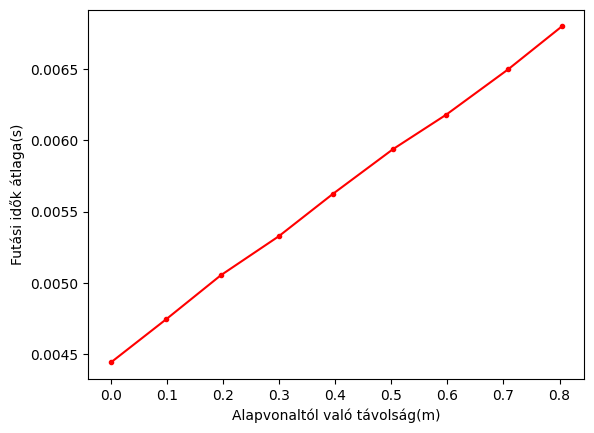
\includegraphics[scale=0.5]{./Valtozo_tavolsag_atlagok.png}
    \caption{Futási idők átlahga az alapvonaltól való távolság függvényében.}
\end{figure}
Ezekre a pontokra egyenest illesztve\footnotemark az egyenes egyenletére a követketkező adódik:
\footnotetext{Az illesztés során az adatpontok hibáját nem lehetett figyelembe venni, mivel azok közül több is 0 volt, így 0-val kellett volna osztani, ami miatt hibás paraméterek adódtak.}
\begin{equation*}
    t=0.00289278\ell+0.00446448
\end{equation*}
Itt a meredekség hibája $\pm2.19567087\cdot 10^{-5}$, a konstans tagé pedig $\pm1.04860417\cdot 10^{-5}$. A hangsebességet az előző egyenes meredekség reciproka adja meg, 
amelyből $c=345.688\frac{m}{s}\pm2.624\frac{m}{s}$ adódik a hangsebességre. Ha az illesztett függvény meredekségét $a$-val jelöljük, akkor a hangsebesség hibájának 
meghatározásához használt képlet a következő:
\begin{equation*}
    \Delta c=\frac{\Delta a}{a}c
\end{equation*}
Amennyiben az illesztést a távolságokra végezzük az idő függvényében az egyenes meredeksége közvetlenül a hangsebességet fogja megadni, amelynek az értéke ilyen bódon számítva:
$c=345.548\frac{m}{s}\pm2.623\frac{m}{s}$ adódik, amely szinte teljes mértékben megegyezik a másik módon kapott eredménnyel. A fent rögzített páratartalomhoz, nyomáshoz 
és hőmérséklethez tartozó hangsebességnek az elméleti számítások szerinti\footnotemark értéke $c=346.26\frac{m}{s}$, amely a mérés során kapott adatokból számolt értékhez 
képest hibahatáron belül van.\footnotetext{A kapott adat a \url{http://resource.npl.co.uk/acoustics/techguides/speedair/} weboldalról származik.}\newline


A rendszer teljes késleltetését úgy haphatjuk meg ha az első illesztés által kapott konstans tagból levonjuk azt az időt, amely ahhoz szökséges, hogy a hang megtegye az 
alapvonal, és a rögzített kapszula közötti távot, melynek nagysága $L_0=1.5495m \pm 0.002 m$. Tehát a késlettetést, és a hibáját a következő képletekkel határozhatjuk meg:
\begin{eqnarray*}
    T_0&=&0.00446448-\frac{L_0}{c} \\
    \Delta T_0&=&=1.04860417\cdot 10^{-5}+\left(\frac{\Delta L_0}{L_0}+\frac{\Delta c}{c}\right)\frac{L_0}{c}
\end{eqnarray*}
Ahol $T_0$ a rendszer teljes késleltetése. Ebből pedig $T_0=-1.789\cdot 10^{-5}s\pm5.0296\cdot 10^{-5}s$ adódik. A fordított illesztésből ezt úgy kaphatjuk meg, hogy a konstans 
tagjához hozzáadjuk $L_0$-t, és elosztjuk $c$-vel, amelyből $T_0=2.01608\cdot 10^{-5}s\pm4.8999\cdot 10^{-5}s$, az itteni számításnál használt képletek:
\begin{eqnarray*}
    T_0&=&\frac{-1.54253346+1.5495}{c} \\
    \Delta T_0&=&\left(\frac{0.0148785+0.002}{-1.54253346+1.5495}+\frac{\Delta c}{c}\right)T_0
\end{eqnarray*}
A kapott késleltetések nagyságrandileg megegyenek az adó, a vevő, és a trigger jelének szélességével, így ez a késleltetés származhat a jelek pontatlan beolvasásából a
mérőpanel által, vagy akár abból is, hogy az ultrahangot nem kezdi el rögtön kibocsájtani a kapszula, amikor megérkeznek bele az adó jelének impulzusai.
\subsubsection*{Doppler-hatás kimutatása}
A mozgatható kapszulát a minimális távolsághoz állítva a ventillátort $12.06V$ feszültség mellett bekapcsoljuk, a termikus egyensúly eléréséhez nagyjából 20 percre volt 
szükség, a hőmérséklet változást az első nagyjából 15 percben az alábbi ábra mutatja:
\begin{figure}[H]
    \centering
    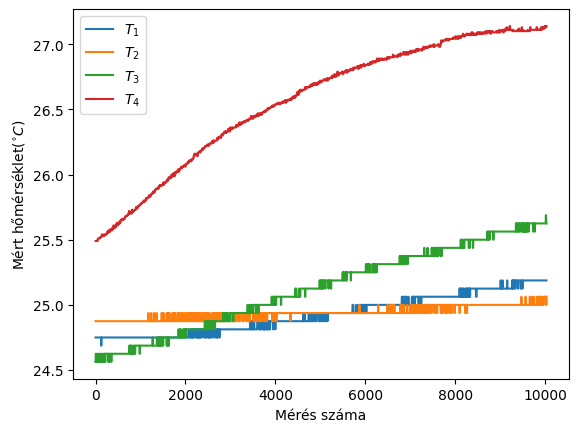
\includegraphics[scale=0.5]{./Ventillator_egyensuly.png}
    \caption{Hőmérők által mért hőmérséklet a ventillátor bekapcsolása után nagyjából 15 percig.}
\end{figure}
Ezen a feszöltségen az oszciloszkóp kurzorainak segítségével leolvassuk a ventillátor fordulatszámát, amely meg meg fog egyezni a ventillátoerból érkező jelen található 
impulzusok frekvenciájával, ebből pedig $f_{12.06}=400.0\pm16 s^{-1}$ \newline


Az egyensúly beálása után a ventillátorba vezetett 3 különböző feszültségérték esetén legalább 1 percig tartó mérést végeztünk, amikből a kapott adatok a szűrés után az alábbiak:
\begin{table}[H]
    \begin{adjustbox}{width=1\textwidth}
        \begin{tabular}{|r|r|r|r|}
            \hline
            Ventillátorba táplált feszültség$(V)$ & Ventillátor fordulatszáma$(s^{-1})$ & Futási idők átlaga$(s)$ & Futási idők szórása$(s)$ \\
            \hline
            8.44 & $303.0\pm8.5$ & 0.00445 & $8.59\cdot 10^{-7}$ \\
            \hline
            12.06 & $400.0\pm16.0$ & 0.00446 & $3.79\cdot 10^{-7}$ \\
            \hline
            13.77 & $463.0\pm8.7$ & 0.00447 & $1.08\cdot 10^{-6}$ \\
            \hline
        \end{tabular}
    \end{adjustbox}
    \caption{Ventillátor fordulatszáma és a futási idők átlaga a betáplált feszültség függvényében.}
\end{table}
\begin{figure}[H]
    \centering
    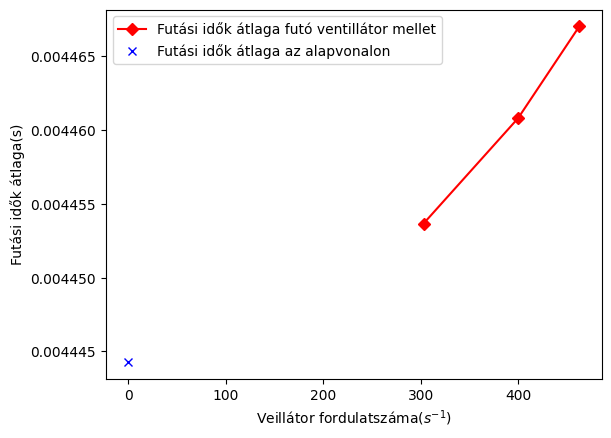
\includegraphics[scale=0.5]{./Doppler.png}
    \caption{Futási idők átlaga a ventillátor fordulatszámának függvényében.}
\end{figure}
A Ventillátor által fújt levegő elsősorban a két T-idom között áramlik, hiszen itt vannak nyitott csapok amelyeken ki és be tud lépni a csőbe. 
Tehát a Doppler jelenség miatt azt várnánk, hogy a terjedési idő átjaga nőjön, ha a levegő és a hang ellentétes irányba mozognak, vagy csökkenjen, ha azonos irányba haladnak. 
A fenti adatokból azt látjuk, hogy a fordulatszám növelésével, amely a levegő áramlási sebességét is növeli valóban nő a terjedési idő, vagyis csökkent a terjedési sebesség.
\subsubsection*{Hőmérők kalibrációja}
Az alábbi ábrán láthatjuk, hogy jogosnak feltételezés a hőmérsékletet állandónak tekinteni, hiszen az általuk mért értékek csak egymáshoz közeli értékek között ugrálnak, 
amely akár a szenzor hibájából is szrmazhat.
\begin{figure}[H]
    \centering
    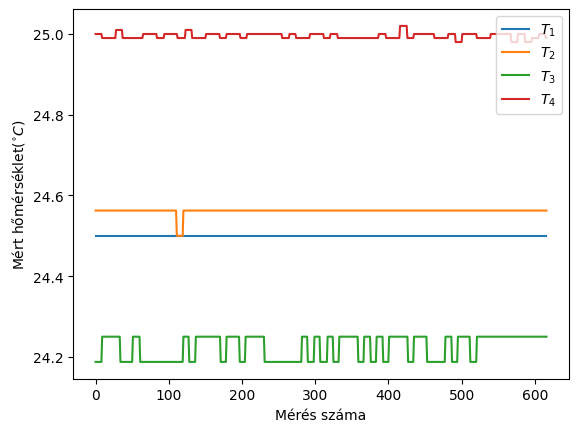
\includegraphics[scale=0.5]{./Homerok.png}
    \caption{Hőmérők által mért adatok az alapvonalon.}
\end{figure}
Az egyes hőmérők által mért hőmérsékletet átlaga pedig a következő:
\begin{table}[H]
    \begin{tabular}{|r|r|}
        \hline
        Hőmérő száma & Hőmérő adatainak átlaga$\left(^{\circ}C\right)$ \\
        \hline
        1. & 24.50 \\
        \hline
        2. & 24.56 \\
        \hline
        3. & 24.22 \\
        \hline
        4. & 25.00 \\
        \hline
        Hőmérők átlaga & 24.57 \\
        \hline
    \end{tabular}
    \caption{Hőmérők Által mért átlag adatok.}
\end{table}
Ebből pedig a hőmérők offsethibáját az adott hőmérő átlaga, és az összes hőmérő átlagának különbségéből kapjuk meg, erre az értékek a következők lesznek:
\begin{table}[H]
    \begin{tabular}{|r|r|}
        \hline
        Hőmérő száma & Hőmérő offsethibája$\left(^{\circ}C\right)$ \\
        \hline
        1. & -0.07 \\
        \hline
        2. & -0.01 \\
        \hline
        3. & -0.35 \\
        \hline
        4. & 0.43 \\
        \hline
    \end{tabular}
    \caption{Hőmérők offsethibája.}
\end{table}
Innentől az összes jegyzőkönyvbe bekerülő hőmérsékleti adat, és azoknak az ábrázolása korrigálva lesz a megfelelő offset hibával.
\subsubsection*{Hangsebesség hőmérsékletfüggése}
Az alábbiakban a következő összefüggést teszteljük:
\begin{equation*}
    c(T)=c_0 \sqrt{\frac{T+T_0}{T_0}}
\end{equation*}
ahol $c$ a hangsebesség értéke $T ^{\circ}C$ hőmérsékleten, $c_0$ a $0^\circ C$ fokon mért hangsebesség, $T_0 \approx 273.15\ ^\circ C$ fok. \newline

Az ultrahangos kapszulát a minimális távolságnál hagyjuk, a kádat elkezdjük vízzel feltölteni. A kád feltöltése során megfigyelhető volt egy ki hőmérsékletváltozás. 
\begin{figure}[H]
    \centering
    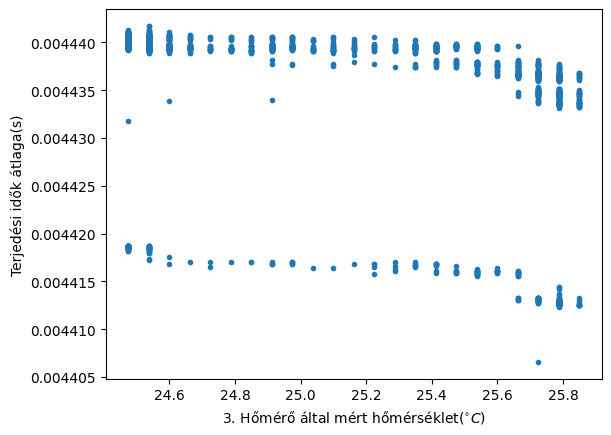
\includegraphics[scale=0.5]{./Feltoltes.png}
    \caption{Mért terjedési idők a feltöltés közben.}
\end{figure}
Mint ahogyan a fenti ábrán is látható itt is problémát fog jelenteni az adatok sávokban való elhelyezkedése, viszont itt nem használhatjuk az előző szűrőrutint, mivel a változás 
során kapott valós adatok nagyját is ki fogja szűrni, ezért kell egy új szűrőalgoritmust írni, amely figyelembe veszi a folyamatos változást, ez a következőt fogja csinálni:
\begin{enumerate}
    \item{Bemeneti értéke egy numpy array, amely tartalmazza a mérési adatokat.}
    \item{Az adatokat a $T_3$-as hőmérséklet alapján növekvő sorrendbe rendezi.}
    \item{Szétbontja az arrayt több kissebb listára, amelyekben egy-egy hőmérsékleti értékhez tartozó adatpontok vannak.}
    \item{Az összes generált listán végigfuttatja az eredezi szűrőrutint.}
    \item{Egyesíti a szűrt listákat, és visszatéríti az egyesített listát.}
\end{enumerate}
\newpage
Ennek a kódja a következő:
\begin{spverbatim}
    def homerseklet_fuggo_szuro(x):
        x = x[x[:,3].argsort()]
        T_jelenlegi = x[:,3][0]
        szakaszok = []
        j = 0
        for i in range(len(x)):
            if x[:,3][i] != T_jelenlegi:
                T_jelenlegi = x[:,3][i]
                szakaszok.append(x[j:i])
                j = i
        eredmeny = []
        for i in range(len(szakaszok)):
            eredmeny.extend(szuro(szakaszok[i]))
        return eredmeny
\end{spverbatim}
A melegítés során kapott adatok ábrázolva a szűrés előtt, és után:
\begin{figure}[H]
    \centering
    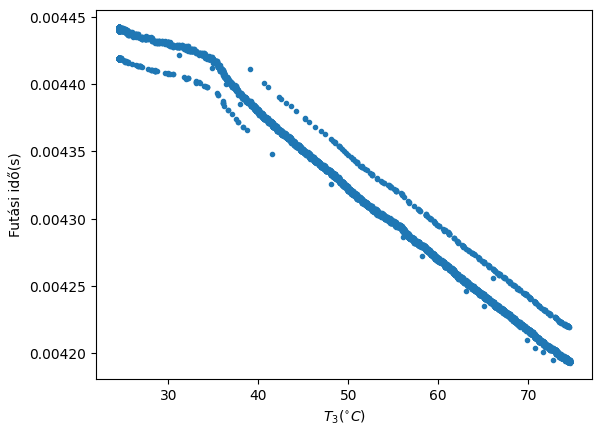
\includegraphics[scale=0.5]{./Szuretlen_melegites.png}
    \caption{Melegítés sotán mért terjedési idők a szűrés előtt.}
\end{figure}
\begin{figure}[H]
    \centering
    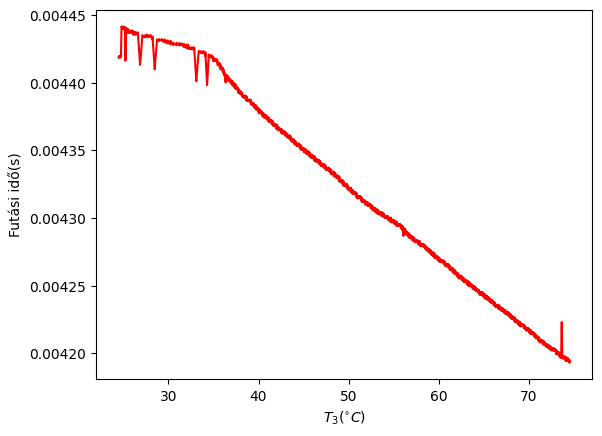
\includegraphics[scale=0.5]{./Szurt_melegites.png}
    \caption{Melegítés sotán mért terjedési idők a szűrés után.}
\end{figure}
Feltételezve, hogy a $45 ^{\circ}C <T_3<70^{\circ}C$ tartományon a kádon belüli csőszakaszban a hőbérséklet értéke megegyezik $T_3$-al, a kádon kívüli szakaszon pedig 
a csőben $T_4$-el a vizsgált képletből a hang terjedési ideje a következő lesz:
\begin{equation*}
    \tau\left(T_3, T_4\right)=\frac{L_{bal}+L_{jobb}}{c_0\sqrt{\frac{T_4+T_0}{T_0}}}+\frac{L_{kád}}{c_0\sqrt{\frac{T_3+T_0}{T_0}}}
\end{equation*}
Ahol $\tau$ a terjedési idő, $L_{bal}=0.248m\pm0.003m$ a kád széle és a bal odlali kapszula, $L_{jobb}=0.231m\pm0.003m$ a kád széle és a jobb oldali kapszula közötti távolság, 
$L_{kád}=1.0705m\pm0.003m$ pedig a kád hossza.
A mért adatok megadott tartományára ezt a függvényt illesztve $c_0=332.607\frac{m}{s}\pm0.015\frac{m}{s}$ és $T_0=267.45 ^{\circ}C \pm0.15 ^{\circ}C$ adódik. A kapott paraméterek 
a valós adatokhoz közel vannak, melyek értéke rendre $c_0=331.5\frac{m}{s}$ és $T_0=273.15\frac{m}{s}$, így jó közelítéssel igaznak tekinthető a vizsgált képlet.
\section*{Összegzés}
A mérések során sikerült hibahatáron belül meghatározni a szoba körülményei között a hangsebességet, valamint kvalitatíve kimutatni a Doppler-hatást. 
Az igazolandó képletnek a paramétereit is jó közelítéssel megkaptuk, így sikerült igazolnunk a képlet helyességét is. Azonban a mérőberendezés feszültségeinek a 
driagrammjain nem látható a trigger jele.
%% IRODALOMJEGYZÉK
%\begin{thebibliography}{9}

%\bibitem{lamport94}
%  Leslie Lamport,
%  \textit{\LaTeX: a document preparation system},
%  Addison Wesley, Massachusetts,
%  2nd edition,
%  1994.
%  \url{https://bla.com}

%\end{thebibliography}

\end{document}